\chapter{Software para Agendamento de Horários de Provas}
\pagestyle{simple}
\label{cap:software}

Para solucionar o problema apresentado no capitulo \ref{cap:problema}, este trabalho irá apresentar uma proposta de “software” que ofereça ao usuário a possibilidade de se agendar horários de prova, de forma simples e obtendo informações necessárias referentes a solução gerada.

Foi definido como objetivo do desenvolvimento, a criação de um “software” que atendesse as seguintes definições:
\begin{enumerate}
    \item[I --] \textbf{Simplicidade}
    
    Buscando ter um sistema que atenda a simplicidade definida por \citeonline[p. 341]{pressman11} como um conteúdo informativo, sucinto, apropriado para as informações entregues. É dito ainda que esse conteúdo deve apresentar uma estética agradável sem exageros, ter sua arquitetura centrada em atender os objetivos da aplicação da maneira mais simples possível e ter uma navegação de forma intuitivamente óbvia.
    
    \item[II --] \textbf{Compatibilidade}
    
\citeonline[p. 342]{pressman11} define como compatibilidade a necessidade da aplicação de ser usada em uma variedade de ambientes distintos (equipamento físico diferentes, categorias de conexão com “internet”, sistemas operacionais, navegadores) e que a mesma deve ser compatível com esses diversos ambientes.
    
    \item[III --] \textbf{Navegabilidade}
    
 A navegação nas páginas deve ser mantida de forma simples, e previsível para \citeonline[p. 342]{pressman11}, visando propiciar ao usuário um comportamento consistente. Os links devem ser sinalizados, e estarem posicionados de forma a facilitar o acesso aos recursos que esses forneçam.
    
    \item[IV --] \textbf{Reusabilidade}
    
Para \citeonline[p. 362]{pressman11} deve-se pensar o sistema de forma a se permitir a reusabilidade, sendo importante por possibilitar a reutilização do programa, ou de parte dele em outras aplicações.  
    
\end{enumerate}


\section{Tecnologias Utilizadas no Desenvolvimento}

\citeonline[p. 35]{pressman11} define como um sistema “web”, uma categoria de “software” centralizada em redes, sendo em sua forma mais simples um conjunto de arquivos de hipertexto interconectados.

Um sistema “web” pode ser dividido em duas partes, chamadas de “Frontend” e “Backend”. \citeonline{mariosouto2019} classifica “frontend” como sendo a parte visual de um sistema, com a qual um usuário pode interagir, e classifica “backend” como a parte do sistema responsável por realizar a ponte entre os dados no navegador e o banco de dados, aplicando regras de negócio e validações, para garantir o acesso às funcionalidades do sistema.

As tecnologias usadas para desenvolver o “Frontend” do protótipo foram:
\begin{itemize}
    \item[] \textbf{HTML 5}   
    
    \begin{citacao} 
    HTML é uma abreviação de “Hypertext Markup Language” - Linguagem de Marcação de Hipertexto. Resumindo em uma frase: o HTML é uma linguagem para publicação de conteúdo (texto, imagem, vídeo, áudio e etc) na Web \cite{ferreiraHTML}.
    
    \end{citacao}     
    A partir da versão 5 muitos novos recursos foram desenvolvidos e disponibilizados, possibilitando maior utilização de elementos visuais na página com uso de apenas HTML.
       
    \item[] \textbf{CSS 3}
    
     O CSS ("Cascading Style Sheet” ou Folhas de Estilo em Cascata em português) é definido por \citeonline{arianegoncalves2019} como uma linguagem de marcação para estilizar páginas HTML.

Em sua versão 3 o CSS se tornou ainda mais compatível com os navegadores moderno e em conjunto do HTML5 possibilitam a criação de elementos que antes seriam necessárias a inclusão de outras linguagens para realização.
   
   
    \item[] \textbf{JavaScript }
      
   O JavaScript é definido por \citeonline{vilsonheckjunior2014} como uma linguagem de “Scripts” que reside dentro de um documento em HTML, promovendo diferentes níveis de interatividade entre o usuário e a página Web, através da Lógica de Programação.

   
    \item[] \textbf{Cytoscape.JS}
    
    É uma biblioteca que utiliza a Teoria dos Grafos escrita em JavaScript de código aberto que permite a visualização, análise de estruturas de Grafos, com elementos animados.
  
   
    \item[] \textbf{Bootstrap}
    \begin{citacao} 
     Bootstrap é uma biblioteca de “frontend” livre e de código aberto para a criação de sites e aplicações “web”. Ele contém HTML e modelos de “design” baseados em CSS para tipografia, formas, botões, navegação e outros componentes da “interface”, bem como extensões JavaScript opcionais. O Bootstrap destina-se a facilitar o desenvolvimento de sites dinâmicos e aplicações “web” \cite{portalgsti2020}.
    
    \end{citacao}    
    
   Com a utilização do Boostrap é possível ter benefícios para o desenvolvedor quanto para o usuário, para o desenvolvedor existirá um padrão que agilizará o desenvolvimento do “software”, para o usuário as páginas possuirão elementos que lembram elementos que ele já utilizou (visualizou) em outras páginas “Web”.
   
\end{itemize}

As tecnologias usadas para desenvolver o “Backend” do protótipo foram:
\begin{itemize}
    \item[] \textbf{PHP 7.0}
       
    PHP (PHP: “Hypertext Processor”) é uma linguagem de “scripts” de código aberto, que se caracteriza por ser embutido em páginas HTML e executado no lado do servidor, sendo usada principalmente para realização de conexões com banco de dados. 
   
    \item[] \textbf{MariaDB 10}
     
     É um Sistema de Gerenciamento de Banco de Dados (SGBD), baseado no MySQL, possuindo todos os comandos, “interfaces”, bibliotecas e APIs existentes no MySQL.
   
    \item[] \textbf{Apache Server}
      
    É um “software” de servidor “web” de código aberto desenvolvido pela \emph{Apache Software Foundation}, que possibilita a comunicação entre um servidor físico e as máquinas dos usuários para realização de transmissão de informações pela “internet”.
   
\end{itemize}

\section{Especificações do Software}



\subsection{Requisitos do Software}

\citeonline[p. 58-59]{sommerville11} define como requisitos de um sistema: as descrições do que o sistema deve fazer, os serviços que oferece e as restrições de funcionamento.

Os requisitos funcionais de “software”, são os serviços que o sistema deve fornecer e como o sistema deve se comportar em cada situação, de acordo com a definição de \citeonline[p. 58-59]{sommerville11}, apresentados a seguir:


\begin{itemize}
    \item[] \textbf{$[$RF001$]$ -- Ler Turmas}

\textbf{Descrição} O “software” deve ler turmas e seus respectivos alunos (entrada).

\item[] \textbf{$[$RF002$]$ -- Ler Horários}

\textbf{Descrição} O “software” deve receber a quantidade de horários disponíveis para prova (entrada).

\item[] \textbf{$[$RF003$]$ -- Gerar Relatório}

\textbf{Descrição} O “software” deve emitir um relatório com os horários de prova por turma (saída).

\item[] \textbf{$[$RF004$]$ -- Gerar Quantidade de Provas de Segunda Chamada}

\textbf{Descrição} O “software” deve informar a quantidade de provas de segunda chamada que necessárias (saída).

\item[] \textbf{$[$RF005$]$ -- Gerar Lista de Alunos em Segunda Chamada}

\textbf{Descrição} Caso existam conflitos de horários o “software” deve informar os alunos e as turmas que precisarão de segunda chamada (saída).

\item[] \textbf{$[$RF006$]$ -- Cadastrar Usuários}

\textbf{Descrição} O “software” deve cadastrar diferentes usuários.

\item[] \textbf{$[$RF007$]$ -- Criar Espaços de Trabalho}

\textbf{Descrição} Os usuários devem poder criar, acessar e modificar seus espaços de trabalho.

\item[] \textbf{$[$RF008$]$ -- Importar Arquivos}

\textbf{Descrição} O “software” deve permitir a importação e exportação de turmas através de arquivos XLSX (planilhas MS Excel).

\item[] \textbf{$[$RF009$]$ -- Gerenciar Espaços de Trabalho}

\textbf{Descrição} O “software” deve permitir separar turmas em diferentes espaços de trabalho.

\item[] \textbf{$[$RF010$]$ -- Autenticar Usuário}

\textbf{Descrição} O “software” deve salvar as informações do usuário mediante a “login” e senha.

\item[] \textbf{$[$RF011$]$ -- Gerenciar Turmas}

\textbf{Descrição} O “software” deve permitir a edição dos dados dos alunos que compõem uma turma.
    
\end{itemize}

\subsection{Regras de Negócio}


A Regra de Negócio é definida como “a forma de fazer o negócio, refletindo a política interna, o processo definido e/ou as regras básicas de conduta” \cite{dextra2013}, serve para estabelecer padrões mínimos de qualidade com base em princípios decididos previamente dos quais as funcionalidades e recursos do sistema devem seguir.


\begin{itemize}
    \item[] \textbf{$[$RN01$]$ -- Estar logado}
    
    \textbf{Descrição} 
    Para utilizar o sistema o usuário precisa ser cadastrado e estar logado.
    
    \item[] \textbf{$[$RN02$]$ -- Turmas devem ter nomes únicos}
    
    \textbf{Descrição}
    Só pode existir uma turma com um determinado nome, caso seja adicionado uma turma com nome igual a uma turma já existente essa inclusão será ignorada. 
    
    \item[] \textbf{$[$RN03$]$ -- Matricula e Nome do Aluno}
    
    \textbf{Descrição}
    Uma matrícula está associada diretamente a um aluno, logo não podem existir dois alunos diferentes com a mesma matrícula, assim como não podem existir duas matrículas para um mesmo aluno.
    
    \item[] \textbf{$[$RN04$]$ -- Disponibilidade de Horário Mínima}
    
    \textbf{Descrição}
    Uma tabela de horário de prova deve ter  no mínimo dois horários disponíveis para realizar os exames.
    
\end{itemize}

\subsection{Casos de Uso}
 
 Casos de Uso são definidos por \citeonline[p. 104]{fowler07} como uma técnica para captar os requisitos funcionais de um sistema, servindo para descrever relações e interações entre usuários e recursos, além de fornecer uma narrativa sobre como o sistema será utilizado.
 
\begin{figure}[h!]
     \centering
     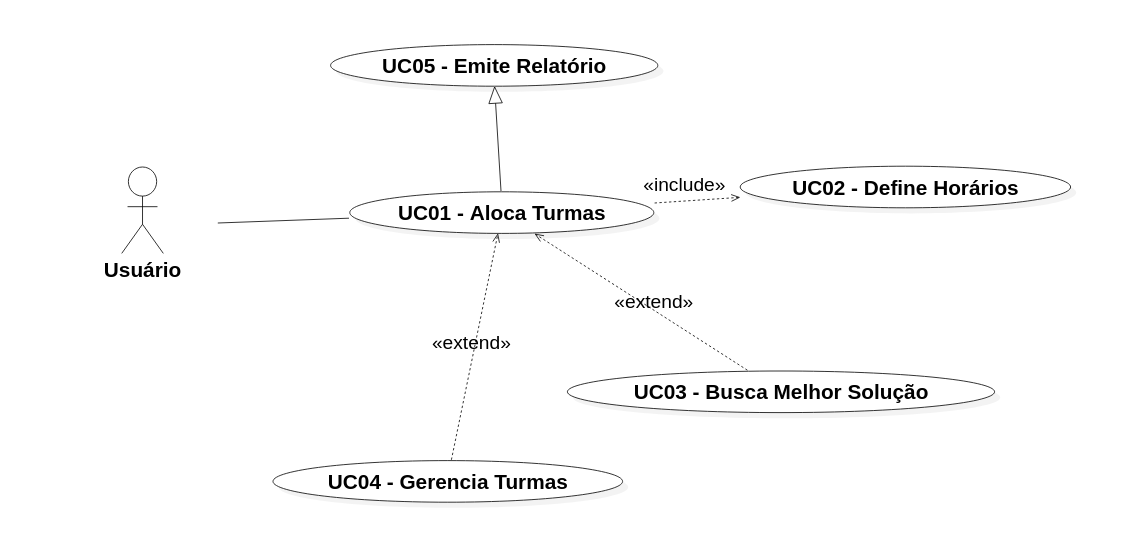
\includegraphics[width=1\textwidth]{TCC/imagens/casodeuso.png}
     \caption{Diagrama de Casos de Uso}
     \label{Diagrama de Casos de Uso}
\end{figure}

 
\subsubsection{Descrição dos Casos de Uso}


\begin{itemize}
    \item[] Descrição dos Atores
    
    \begin{itemize}
        \item[$\ast$] \textbf{Usuário}
        
        \textbf{Descrição} 
        
        Toda pessoa ou “software” que irá interagir com o sistema através de sua “interface” gráfica.
    \end{itemize}
    
    \item[] Casos de Uso
    
    \begin{itemize}
        \item[$\ast$] \textbf{$[$UC01$]$ -- Aloca Turmas}
        
        \textbf{Descrição}
        
         Este caso de uso permite que o usuário possa definir horários específicos de prova para alocar as turmas.
        
        \textbf{Pré-condições}
        \begin{enumerate}
            \item O usuário deve estar logado.
            \item O usuário deve ter turmas e seus respectivos alunos cadastrados no sistema.
            \item O usuário deve definir a quantidade de horários disponíveis para realização das provas.
        \end{enumerate}
       
        \textbf{Pós-condições}
        \begin{enumerate}
            \item  O sistema deve atribuir cada turma á um único horário.
            \item  O sistema deve informar a quantidade total de conflitos de alunos em duas turmas em um mesmo horário.
        \end{enumerate}
       
        
        \begin{table}[H]
            \centering
            \caption{Fluxo Principal de Interações de $[$UC01$]$}
            \vspace{0.5cm}
            \renewcommand\arraystretch{1.5}
            \begin{tabular}{c|p{6cm}|p{6cm}}
             
                \textbf{Sequência} & \textbf{Usuário} & \textbf{Sistema} \\ % Note a separação de col. e a quebra de linhas
                \hline                               % para uma linha horizontal
                1 & Seleciona uma turma e move para uma caixa de horário.  &  \\
                2 &   & Atribui a turma á um horário. \\
                3 & & Calcula o número de alunos que tenham duas provas em um mesmo de horário.          % não é preciso quebrar a última linha
                \\
                \hline
            \end{tabular}
        \end{table}
        
       
        
        \item[$\ast$] \textbf{$[$UC02$]$ -- Define Horários}
        
        \textbf{Descrição}
        
        Este caso de uso realiza a leitura da quantidade de horários de prova que o usuário dispõe para a realização das provas.
        
        \textbf{Pré-condições}
        \begin{enumerate}
            \item  O usuário deve estar logado. 
        \end{enumerate}
        
        \textbf{Pós-condições}
        \begin{enumerate}
            \item O sistema deve registrar como quantidade de horários um número maior ou igual a dois. 
            \item O sistema deve permitir a execução do caso de uso $[$UC01$]$.
        \end{enumerate}
        
     \begin{table}[H]
            \centering
            \caption{Sequência de Interações de $[$UC02$]$}
            \vspace{0.5cm}
            \renewcommand\arraystretch{1.5}
            \begin{tabular}{c|p{6cm}|p{6cm}}
             
                \textbf{Sequência} & \textbf{Usuário} & \textbf{Sistema} \\ % Note a separação de col. e a quebra de linhas
                \hline                               % para uma linha horizontal
                1 & Informa a quantidade de horários de prova disponível.  &  \\
                2 &   & Atualiza o número de caixas de horários.
                \\
                \hline
            \end{tabular}
        \end{table}
        
        \item[$\ast$] \textbf{$[$UC03$]$ -- Busca Melhor Solução}
        
        \textbf{Descrição}
        
        Este caso de uso permite ao sistema a executar um algoritmo de modo a buscar automaticamente uma alocação com o menor custo possível para as turmas selecionadas.
        
        \textbf{Pré-condições}
        \begin{enumerate}
            \item  O caso de uso $[$UC01$]$ deve ter sido executado.
            \item  O usuário precisa indicar todas as turmas que deverão realizar as provas nos horários indicados.
        \end{enumerate}
        
        \textbf{Pós-condições}
        \begin{enumerate}
            \item  O sistema deve encontrar a alocação que resulte no menor número de provas de segunda chamada forçadas pela alocação.
            \item O sistema deve encaminhar automaticamente o usuário para o caso de uso $[$UC05$]$.
        \end{enumerate}
        
        \begin{table}[H]
            \centering
            \caption{Fluxo Principal de Interações de $[$UC03$]$}
            \vspace{0.5cm}
            \renewcommand\arraystretch{1.5}
            \begin{tabular}{c|p{6cm}|p{6cm}}
             
                \textbf{Sequência} & \textbf{Usuário} & \textbf{Sistema} \\ % Note a separação de col. e a quebra de linhas
                \hline                               % para uma linha horizontal
                1 & Seleciona a opção de buscar a melhor solução.  &  \\
                2 &   & Executa algoritmo para buscar solução ideal. \\
                3 & & Redireciona para tela de Relatório com a solução ideal.          % não é preciso quebrar a última linha
                \\
                \hline
            \end{tabular}
        \end{table}
        
        \item[$\ast$] \textbf{$[$UC04$]$ -- Gerencia Turmas}
        
        \textbf{Descrição}
        
        Este caso de uso permite que o usuário crie, edite, remova, importe e exporte turmas, e seus respectivos alunos dentro do sistema.
        
        \textbf{Pré-condições}
        \begin{enumerate}
            \item  O usuário deve estar logado.
        \end{enumerate}
        
        \textbf{Pós-condições}
        \begin{enumerate}
            \item  O sistema deve atualizar o banco de dados com as novas informações assim que alteradas pelo usuário.
            \item  O sistema deve permitir alterações de forma simplificada pelo usuário.
            \item  O sistema deve exibir mensagens de alerta para o usuário em caso de alterações que não possam ser desfeitas.
        \end{enumerate}
        
       \begin{table}[H]
            \centering
            \caption{Fluxo de Interações de $[$UC04$]$ -- Criação de Turma}
            \vspace{0.5cm}
            \renewcommand\arraystretch{1.5}
            \begin{tabular}{c|p{6cm}|p{6cm}}
             
                \textbf{Sequência} & \textbf{Usuário} & \textbf{Sistema} \\ % Note a separação de col. e a quebra de linhas
                \hline                               % para uma linha horizontal
                1 & Seleciona a opção de “Adicionar Turma” na página de gerenciamento de turmas  &  \\
                2 &   & Redireciona a página atual para a página de “Criação de Turmas”  \\
                3 & Informa o nome da turma que deseja criar &    \\
                4 & Seleciona a opção para inserir o aluno & \\ 
                5 & & Cria a opção de inclusão de matrícula e nome para o novo aluno \\
                6 & Informa a matrícula e o nome do aluno & \\
                7 & Seleciona a opção “Criar Turma” & \\
                8 & & Grava turma no banco de dados \\ 
                9 & & Vincula alunos á turma criada \\
                10 & & Redireciona a página atual para a página de “Gerenciamento de Turmas"
                % não é preciso quebrar a última linha
                \\
                \hline
            \end{tabular}
        \end{table}
        
        \begin{table}[H]
            \centering
            \caption{Fluxo de Interações de $[$UC04$]$ -- Visualização de Turma}
            \vspace{0.5cm}
            \renewcommand\arraystretch{1.5}
            \begin{tabular}{c|p{6cm}|p{6cm}}
             
                \textbf{Sequência} & \textbf{Usuário} & \textbf{Sistema} \\ % Note a separação de col. e a quebra de linhas
                \hline                               % para uma linha horizontal
                1 & Seleciona a opção de “Visualizar” de uma turma  &  \\
                2 & & Redireciona a página atual para a página de “Visualização de Turma” \\
                3 & & Exibe uma lista em ordem alfabética com os alunos da turma         % não é preciso quebrar a última linha
                \\
                \hline
            \end{tabular}
        \end{table}
        
        \begin{table}[H]
            \centering
            \caption{Fluxo de Interações de $[$UC04$]$ -- Edição de Turma}
            \vspace{0.5cm}
            \renewcommand\arraystretch{1.5}
            \begin{tabular}{c|p{6cm}|p{6cm}}
             
                \textbf{Sequência} & \textbf{Usuário} & \textbf{Sistema} \\ % Note a separação de col. e a quebra de linhas
                \hline                               % para uma linha horizontal
                1 & Seleciona a opção de “Editar” uma turma  &  \\
                2 & & Redireciona a página atual para a página de “Edição de Turma” \\
                3 & & Exibe uma lista em ordem alfabética com os alunos da turma \\
                4 & & Habilita os campos de matrícula e nome para edição \\
                5 & Altera o nome e a matricula de um aluno & \\
                6 & Seleciona a opção “Salvar Alterações” & \\
                7 & & Atualiza a lista de alunos pertencentes á turma no banco de dados \\
                8 & & Redireciona a página atual para página de “Gerenciamento de Turmas” 
                % não é preciso quebrar a última linha
                \\
                \hline
            \end{tabular}
        \end{table}
        
        \begin{table}[H]
            \centering
            \caption{Fluxo de Interações de $[$UC04$]$ -- Exclusão de Turma}
            \vspace{0.5cm}
            \renewcommand\arraystretch{1.5}
            \begin{tabular}{c|p{6cm}|p{6cm}}
             
                \textbf{Sequência} & \textbf{Usuário} & \textbf{Sistema} \\ % Note a separação de col. e a quebra de linhas
                \hline                               % para uma linha horizontal
                1 & Seleciona a opção de “Apagar” uma turma  &  \\
                2 &   & Exibe um alerta \\
                3 & Seleciona a opção “Sim” no alerta &   \\
                4 & & Apaga a turma do banco de dados \\
                5 & & Atualiza a página de “Gerenciamento de Turmas"
                % não é preciso quebrar a última linha
                \\
                \hline
            \end{tabular}
        \end{table}
        
        \item[$\ast$] \textbf{$[$UC05$]$ -- Emite Relatório}
        
        \textbf{Descrição}
        
        Este caso de uso permite que o usuário visualize de forma gráfica os resultados e informações referentes a alocação feita, como a quantidade de alunos prejudicados pela alocação, e a lista de alunos que foram prejudicados.
        
        \textbf{Pré-condições}
        \begin{enumerate}
            \item  O caso de uso $[$UC01$]$ ou o caso de uso $[$UC02$]$ devem ter sido executados.
        \end{enumerate}
        
        \textbf{Pós-condições}
        \begin{enumerate}
            \item O sistema deve informar a quantidade de conflitos gerados pela alocação.
            \item O sistema deve informar os alunos prejudicados com duas provas alocadas em um mesmo horário.
            \item O sistema deve permitir o “download” e/ou impressão do relatório através de arquivo PDF.
        \end{enumerate}
        
       \begin{table}[H]
            \centering
            \caption{Fluxo Principal de Interações de $[$UC05$]$}
            \vspace{0.5cm}
            \renewcommand\arraystretch{1.5}
            \begin{tabular}{c|p{6cm}|p{6cm}}
             
                \textbf{Sequência} & \textbf{Usuário} & \textbf{Sistema} \\ % Note a separação de col. e a quebra de linhas
                \hline                               % para uma linha horizontal
                1 & Conclui a alocação das turmas em seus respectivos horários para realizarem as provas.  &  \\
                2 &   & Exibe a quantidade de provas de segunda chamada necessárias com a alocação.       \\
                3 & & Exibe a alocação feita.     \\
                4 & & Fornece a opção de gerar PDF do relatório. \\ 
                5 & & Fornece a opção de realizar nova alocação. % não é preciso quebrar a última linha
                \\
                \hline
            \end{tabular}
        \end{table}
        
    \end{itemize}
    
\end{itemize}




\subsection{Diagrama de Atividades}
 
 O diagrama de atividades auxilia na criação e representação de um fluxo de utilização de um sistema por um usuário.
 
 O diagrama \ref{Diagrama Atividades} apresenta o comportamento do sistema a medida em que um usuário acessa suas funcionalidades, iniciando em sua  primeira conexão ao sistema até a impressão do relatório contendo o resultado obtido com a alocação realizada.
 
 \begin{citacao}
     Os diagramas de atividades são uma técnica para descrever lógica de procedimento, processo de negócio e fluxo de trabalho. De várias formas, eles desempenham um papel semelhante aos fluxogramas, mas a principal diferença entre eles e a notação de fluxograma é que os diagramas suportam comportamento paralelo. \cite[p. 118]{fowler07}
 \end{citacao}
 
\begin{figure}[H]
     \centering
     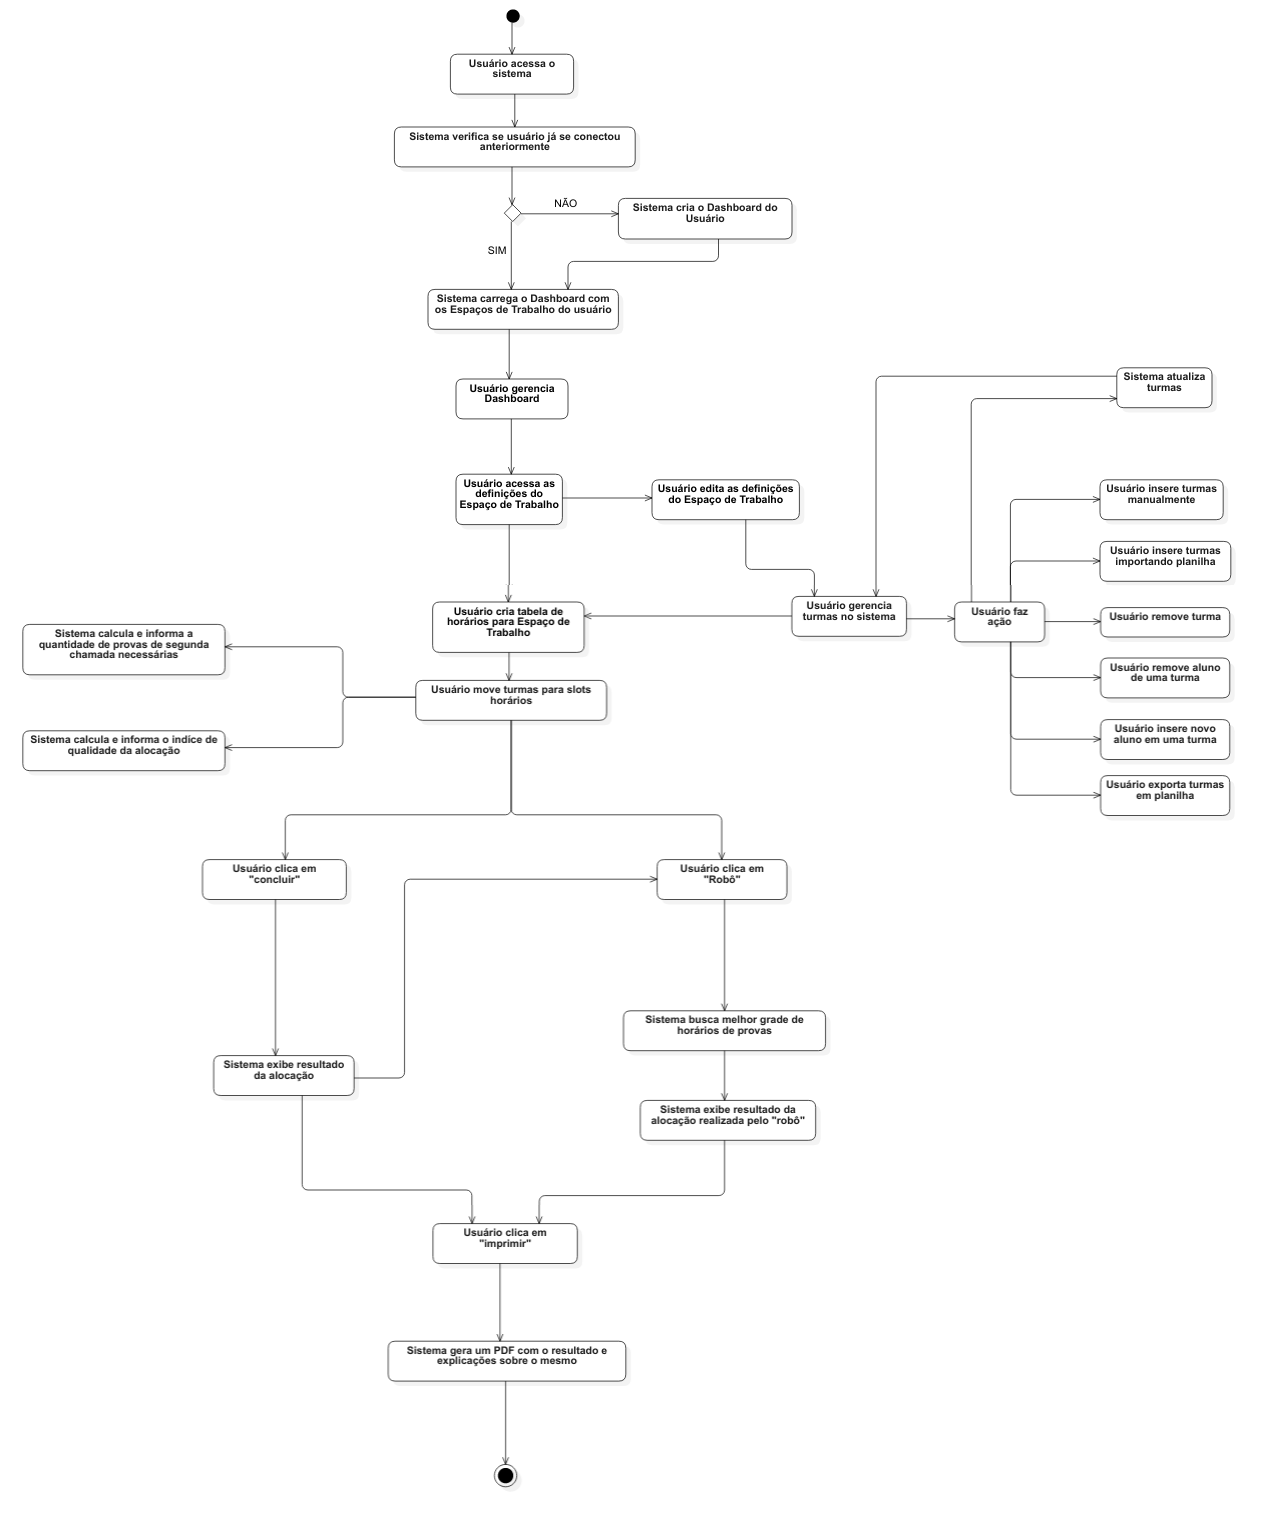
\includegraphics[width=1.1\textwidth]{TCC/imagens/atividades.png}
     \caption{Diagrama de Atividades}
     \label{Diagrama Atividades}
\end{figure}

 
 
\subsection{Diagrama de Classes}

O diagrama de classes é um dos diagramas mais utilizados em UML, ele apresenta a forma pela qual o código está estruturado, permitindo dessa forma, que outros desenvolvedores possam compreender o funcionamento do “software”, facilitando dessa maneira a organização do código e sua manutenção ao longo do tempo.

% O diagrama apresentado em \ref{Diagrama de Classes} consiste na utilização das classes \emph{usuário}, que será responsável por interagir com o sistema, \emph{espaço de trabalho}, qe poderá representar tanto uma instituição quanto um grupo de turmas, \emph{turmas}, e seus respectivos \emph{alunos}, e a \emph{grade de provas} que consiste no controle do resultado e a alocação.

 \begin{citacao}
      Um diagrama de classes descreve os objetos presentes no sistema e os vários relacionamentos estáticos existentes entre eles. Os diagramas de classes também mostram as propriedades e as operações de uma classe e as restrições que se aplicam à maneira como os objetos estão conectados. A UML utiliza a palavra característica como um termo geral que cobre as propriedades e operações de uma classe. \cite[p. 52]{fowler07}
 \end{citacao}
 
\begin{figure}[H]
     \centering
     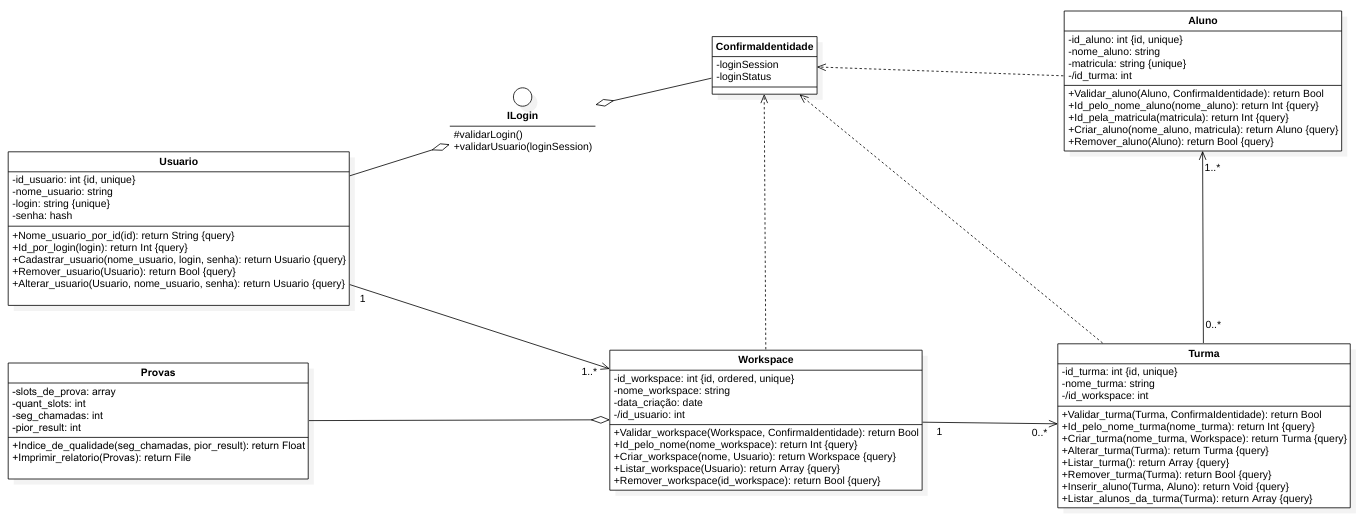
\includegraphics[width=1.4\textwidth,angle=270]{TCC/imagens/classes.png}
     \caption{Diagrama de Classes}
     \label{Diagrama de Classes}
\end{figure}


\subsection{Diagrama de Entidade-Relacionamento}

O diagrama de entidade-relacionamento é utilizado para permitir a representação geométrica das relações entre diferentes entendidas abstratas, podendo essas serem pessoas, cargos, objetos, imóveis e quaisquer outros conjuntos que possuam atributos em comum que os permita serem diferenciados.

O diagrama neste trabalho apresenta as relações entre turmas e seus respectivos alunos, as turmas que compõem um espaço de trabalho (\textit{workspace}), que representarão um conjunto de turmas,  por exemplo uma instituição ou turno, e dessa forma a relação entre um usuário e todos os seus espaços de trabalho.

  \begin{citacao}
   A técnica de modelagem de dados mais difundida e utilizada é a abordagem entidade-relacionamento (ER). Nesta técnica, o modelo de dados é representado através de um modelo entidade-relacionamento (ER). Usualmente, um modelo ER é representado graficamente, através de um diagrama entidade-relacionamento (DER). A abordagem ER foi criada em 1976 por Peter Chen. Ela pode ser considerada um padrão de fato para modelagem conceitual. \cite[p. 12]{heuser09}
    \end{citacao}
    
\begin{figure}[!h]
     \centering
     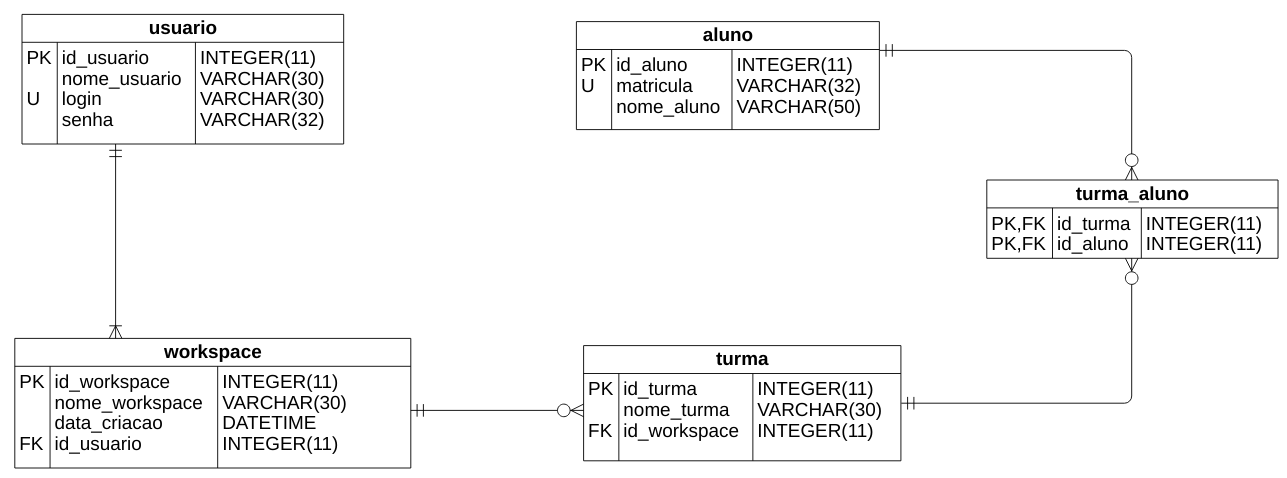
\includegraphics[width=1\textwidth,angle=270]{TCC/imagens/DER.png}
     \caption{Diagrama de Entidade Relacionamento}
     \label{Diagrama de Entidade Relacionamento}
\end{figure}
 
% \subsection{Diagrama de Fluxo de Telas}

\subsection{Relatórios}

O relatório gerado pelo sistema tem como propósito ser um documento para o usuário com as informações referentes a forma como as turmas foram distribuídas, possíveis conflitos causados pela alocação, e explicações sobre a construção e funcionamento do sistema.

Seu foco é: ser instrutivo, de modo a permitir que o usuário consiga replicar o resultado em uma universidade real. Ser didático, visando explicar as bases do problema matemático por trás do problema de horários de exames universitários e a proposta de solução usada no trabalho.

A partir do arquivo PDF gerado pelo sistema, é possível efetuar o “download” do relatório e salva-lo digitalmente, e também permite a impressão do mesmo, caso seja desejável ter uma versão física da solução.

Dessa forma o relatório serve tanto como uma instrução de como a grade de prova poderá ser realizada, como um documento com propósito explicativo que justifique a alocação e que antecipe os problemas que por ventura venham a acontecer, no caso os alunos com mais de uma prova em um mesmo horário.